\PassOptionsToPackage{svgnames}{xcolor}
\documentclass[a4paper,14pt]{article}

\input preamble.tex

\usepackage{sectsty}
\usepackage{lipsum}
\usepackage{indentfirst}
\allsectionsfont{\centering\normalsize} % Заголовки с абзацного отступа: \indent %% по центру \centering
\subsectionfont{\normalsize\centering} % Подразделы с абзацного отступа + обычный шрифт

\begin{document}
\thispagestyle{empty}
\begin{center}
	Министерство сельского хозяйства РФ \\Федеральное государственное бюджетное образовательное учреждение\\ высшего образования
	\vspace{0.5ex}
	
	<<Пермский государственный аграрно-технологический университет\\ имени академика Д.Н. Прянишникова>>
\end{center}
\vspace{10ex}
\begin{tabularx}{\textwidth}{XX}
	& Кафедра организации производства  \\
	& и предпринимательства в АПК
\end{tabularx}
\begin{center}
	\vspace{13ex}
	Контрольная работа\\
	по дисциплине <<Экономическая оценка инвестиций>> \\
%	\vspace{1ex}
%	на тему <<Экономическая эффективность инвестиционной\\ деятельности предприятия на примере ООО <<Агрофирма Острожка>>
%	\vspace{1ex}
	
%	Вариант 3
\end{center}
	\vspace{8ex}
	\begin{tabularx}{\textwidth}{XX}
	& Выполнил:\\
	& студент факультета заочного \\
	& обучения по направлению \\
	& <<Менеджмент>> \\
	& Кузнецов Андрей Валерьевич \\
	& Шифр Мн-13-204\\
	& Руководитель:\\
	& к.э.н., доцент\\
	& Серогодский Владимир Эдуардович\\
	\end{tabularx}
\begin{center}
	\vfill
	Пермь 2018
\end{center}

\newpage
%\thispagestyle{empty}
%\begingroup
%	\centering{
		\tableofcontents
				%}
%\endgroup
			
		%

%\newpage
%\subsection*{Введение}
\addcontentsline{toc}{section}{Введение}


\newpage
\section{Теоретические вопросы}
\subsection{Характеристика инвестиционного климата в России. Факторы, определяющие инвестиционный климат}

Высокая инвестиционная активность --- одно из условий развития экономики страны.
Она достигается за счет роста объемов реализуемых инвестиционных ресурсов и их целесообразного использования в различных сферах.
Инвестиции на новой научно-технической базе формируют производственный потенциал конкретной организации в целом, предопределяют конкурентные позиции России на мировых рынках.
Важную роль играет возможность привлечения иностранного капитала в виде прямых капиталовложений, портфельных инвестиций и других активов.
Это выполнимо только при условии хорошего инвестиционного климата в стране.

Инвестиционный климат --- совокупность  политических. экономических, юридических, социальных, бытовых и других факторов, которые предопределяют степень риска капиталовложений и возможность их эффективного использования.
инвестиционный климат зависит от инвестиционной активности и инвестиционной привлекательности (см. \ref{fig:invest})

\begin{figure}[h]
	\centering
	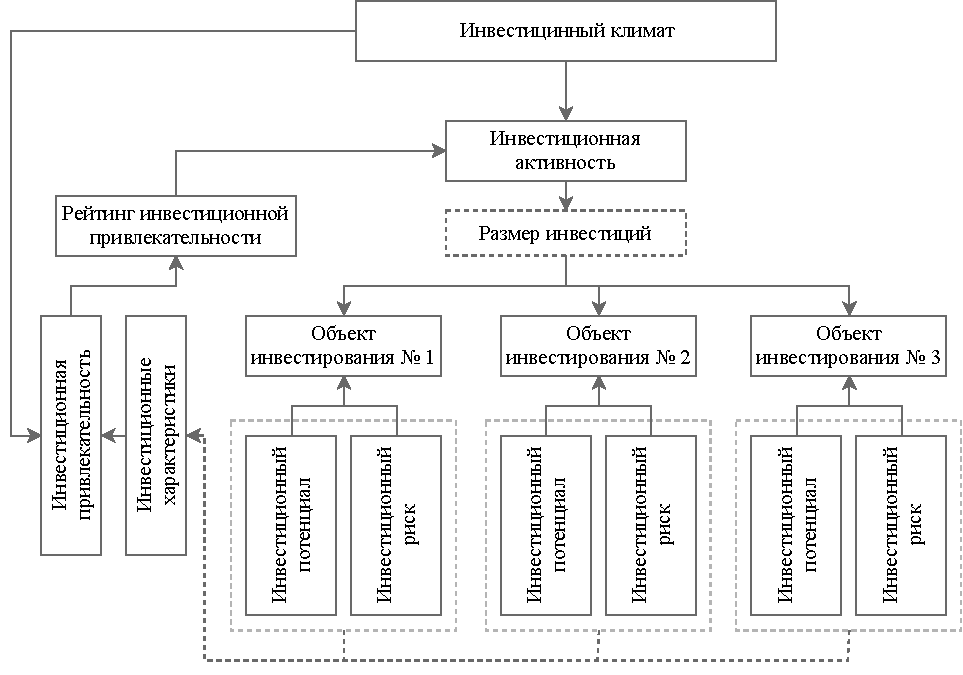
\includegraphics[width=1\linewidth]{invest}
	\caption{Взаимосвязь между инвестиционным климатом, инвестиционной активностью и инвестиционной привлекательностью}
	\label{fig:invest}
\end{figure}

Под инвестиционной активностью понимается динамика размера, структуры инвестиций, а также эффективность их использования.
Она напрямую зависит от рейтингов объектов инвестирования, публикуемых рейтинговыми агентствами и консалтинговыми компаниями.
В настоящее время рассчитываются рейтинги стран, субъектов федерации, городов и организаций.
Ключевое влияние на рейтинг оказывает инвестиционная привлекательность.
Она выражается в наборе качественных характеристик, делающих потенциальный объект  инвестирования безопасным и выгодным вложением для инвесторов.
Рейтинг может быть представлен с помощью индекса, на основе которого сравниваются объекты со схожими качественными характеристиками.

Степень инвестиционной привлекательности объекта зависит от инвестиционного потенциала и инвестиционного риска.
Она определяется совокупностью имеющихся объективных показателей и предпосылок для осуществления инвестиций (инвестиционный потенциал), а также вероятностью возникновения непредвиденных финансовых потерь в условиях неопределенности вложения капитала за счет изменения макроэкономической ситуации (инвестиционный риск).
Степень инвестиционной привлекательности отражается на размере инвестиций в различные объекты.

Российские исследователи выделяют следующие факторы, оказывающие влияние на инвестиционный климат:
\begin{itemize}
	\setlength\itemsep{0pt}
	\item политическая стабильность;
	\item нормативно-законодательная база и скорость ее изменения;
	\item состояние внутреннего рынка страны и ее финансовой системы;
	\item размер налогового бремени;
	\item платежеспособный спрос населения;
	\item квалификация персонала;
	\item стоимость ресурсов (сырьевых, трудовых, финансовых);
	\item информационное обеспечение;
	\item задолженность по внешним обязательствам перед международными экономическими и финансовыми организациями.
\end{itemize}

Согласно существующим критериям Россия в настоящее время относится к государствам со средним уровнем достигнутого экономического развития  и умеренными инвестиционными рисками.

Привлекательность вложения в страну финансовых средств определяется индексами деловой активности фондового рынка: в США --- DowJones и NASDAQ, в Европе --- EuroCtoxx 50,  в том числе FTSE (Лондон), XETRA DAX (Франкфурт-на-Майне), CAC-40 (Париж), SMI (Цюрих), AEX (Амстердам), MIBTel (Милан), IBEX (Мадрид), в Японии --- Nikke1-225, в Китае --- HANGSENQ, в России --- ММВБ-РТС и др.

Решение об инвестировании принимается после оценки инвестиционного климата страны и отдельного региона, в который планируется осуществить вложения.
В настоящее время разработаны и применяются следующие методики оценки инвестиционного климата:

1) универсальная методика оценки инвестиционного климата включает в себя максимальное количество экономических характеристик, показателей торговли, характеристик политического климата и законодательства.
Такая информационная база позволяет провести корректную оценку ситуации в стране на текущий момент и сделать прогноз относительно ее развития;

2) методика сравнительного анализа инвестиционного климата используется в государствах с переходной экономикой.
Ее основу составляют специализированные методики, позволяющие сделать акцент на темпах и перспективах реформ.
Информационной основой анализа являются данные опроса экспертов, представляющих крупные банки развитых стран.
Кроме этого, методика учитывает статистическую информацию о состоянии того или иного фактора развития экономики;

3) методика бальной оценки.
Она позволяет провести количественное сопоставление основных характеристик инвестиционного климата стран и определить показатели, которые учитывают величины всех составляющих и служат критерием ранжирования стран по их инвестиционной привлекательности.

Оценить инвестиционный климат России непросто.
Основная проблема, которая возникает при проведении оценки --- это наличие большой территории с различными климатическими условиями, природными ресурсами и другими факторами.
Поэтому чаще всего оценивают инвестиционный климат отдельных регионов, а не страны в целом.

В России существует большая дифференциация между регионами: существуют регионы, которые живут за счет субсидий из федерального бюджета, и регионы-доноры.

Ключевую роль на российском рынке оценки инвестиционного климата регионов занимает рейтинговое агентство <<Эксперт РА>>.
В качестве информационной базы агентство использует ежегодно собираемые по типовой методике данные Федеральной службы государственной статистики РФ, Министерства финансов РФ, министерства экономического развития РФ, Центрального банка РФ, Федеральной налоговой службы, Министерства внутренних дел РФ, а также базы новостных лент российских информационных агентств и собственные базы данных.
При оценке законодательного риска используется справочная правовая система <<КонсультантПлюс>>.
Для оценки распространения сотовой связи и интернета используются данные компании iKS-Consulting, результаты федеральных и региональных выборов публикуются на интернет-сайтах Центризбиркома РФ и избирательных комиссий субъектов Федерации.
При составлении рейтинга также используется информация по законодательству, стратегиям и программам регионального развития, представленная на сайтах регионов, а также предоставленная агентству администрациями отдельных субъектов Федерации по собственной инициативе.

Инвестиционная привлекательность в рейтинге оценивается по двум параметрам: инвестиционному потенциалу и инвестиционному риску.

Потенциал показывает, какую долю регион занимает на общероссийском рынке, риск --- какими могут быть для инвестора масштабы тех или иных проблем в регионе.
Суммарный потенциал состоит из девяти частных: трудового, финансового, производственного, потребительского, институционального, инфраструктурного, природно-ресурсного, туристического и инновационного.

Интегральный риск состоит из шести частных: финансового, социального, управленческого, экономического, экологического и криминального.
Вклад каждого частного риска или потенциала в итоговый индикатор оценивается на основе анкетирования представителей экспертного, инвестиционного и банковского сообществ.

Рейтинг инвестиционной привлекательности регионов России 2017 года впервые за долгое время демонстрирует снижение интегрального инвестриска и всех его частных составляющих. Самая острая фаза кризиса пройдена и в показателях 2016-го, это отразилось в сокращении интегрального инвестиционного риска на 3,1\% относительно уровня 2015 года. Наибольшее снижение у финансового риска (-4,8\%), а наименьшее – у управленческого (-1,2\%).

Произошедшее в кризис размывание понятного набора рычагов воздействия на экономический рост требует от региональных властей усложнения управленческого инструментария. Волна отставок и назначений в губернаторском корпусе свидетельствует, что ответ на новые вызовы оказались способны найти далеко не все руководители территорий. Из анализа рейтинга необходимость перемен в составе региональных команд вытекает вполне четко: почти в 2/3 субъектов Федерации, где произошла смена губернатора, показатели социальных, финансовых и экономических рисков по итогам 2014–2016 годов были заметно хуже средних.

Благодаря агломерационному эффекту первыми частичное выправление ситуации почувствовали крупнейшие экономические центры страны. В нынешнем рейтинге 12 из 17 регионов, в состав которых входят города-миллионники, включая пристоличные области (Московская и Ленинградская), улучшили свое положение по показателю интегрального риска. Так, Петербург прибавил 3 позиции, Новосибирская область – 6, Волгоградская – целых 10, а Московская – 4, выйдя в лидеры списка.

Рейтинг показывает, что многим регионам предстоит пережить смену экономической парадигмы. Если до кризиса роль тех или иных региональных драйверов была очевидной для конкретных территорий, то сейчас картина социально-экономического развития в региональном преломлении стала расфокусированной. Так, Ростовская область, считающаяся по преимуществу аграрной, в нынешнем рейтинге поднялась на 3 позиции в первую очередь за счет машиностроительных предприятий, равно как и традиционно индустриальные Иркутская и Ульяновская области – плюс 4 и 3 позиции соответственно.

Нынешний рейтинг отражает постепенное прекращение живительного воздействия инъекций «нефтяной иглы». Заметно сдали позиции Ханты-Мансийский автономный округ – Югра (минус 8 мест по риску) и Омская область (минус 5).

Влияние агропромышленного комплекса после очевидного эффекта, вызванного девальвацией, ослабло. Из-за неблагоприятной мировой ценовой конъюнктуры, способствовавшей снижению экспорта, в 2016 году показатели ряда мощных зерновых регионов страны просели с точки зрения инвестпривлекательности. Это стало одной из причин перемещения Краснодарского края с 1-й строчки на 4-ю по интегральному инвестриску и Ставрополья с 16-й позиции на 24-ю. Схожую динамику в рейтинге показал и ряд областей Центрального Черноземья: Тамбовская (5-е место против 2-го годом ранее), Курская (10-е и 6-е) и Орловская (62-е и 58-е). Лучше в рейтинге показали себя регионы, где в последнее время идет активное наращивание производства и переработки говядины (вложения в производство свинины и мяса птицы сыграли свою роль в прошлые годы), – это прежде всего Белгородская (переход с 8-го места в прошлом рейтинге на 7-е в нынешнем) и Брянская (31-я и 36-я позиции соответственно) области. Тем не менее, потенциал развития АПК и его влияния на экономики территорий далек от исчерпания, в том числе и в связи с продолжающейся господдержкой сектора.

На выходе из кризиса заметно снизилось стимулирующее воздействие на региональные экономики федеральных программ. Наиболее показательны в этом отношении Крым и Севастополь – в нынешнем рейтинге эти два региона переместились вниз на 5 и 6 позиций соответственно из-за очевидных сбоев в управлении, выразившихся в неспособности осваивать бюджетные средства и вовлекать местный бизнес в реализацию крупных проектов. Снижение эффекта от бюджетных вливаний на экономику продемонстрировала и Амурская область (падение на 16 позиций по интегральному показателю риска) из-за паузы в строительстве следующих очередей космодрома Восточный.

Предпосылки для роста региональных экономик создало проведенное государством оздоровление региональных бюджетов. После долгих лет неизменного роста началось сокращение долговой нагрузки на бюджеты субъектов РФ, которое сопровождалось и оздоровлением структуры долга: за январь – сентябрь 2017 года портфель банковских кредитов региональным бюджетам сократился на 33\%, почти половина от этого сокращения – заслуга займов из федерального бюджета. При осмысленном выборе приоритетов и грамотной экономической политике средства, не потраченные на погашение высоких процентов по коммерческим кредитам, можно будет пустить на развитие.












\subsection{Принципы оценки эффективности инвестиционного проекта}
\subsection{Основные мероприятия, направленные на снижение инвестиционных рисков в проектах}
%\input{1-3glava}

%\section{Автоматизированные методы распределения в коммерческой логистике}
\subsection{1}


%\newpage
%\section{Алгоритм формирования складской сети}
\subsection{1}


\newpage
\section{Задачи}
\subsection*{Задача 1}
Предприятие через 6 лет желает иметь на счете 1600 тыс. руб. Для этого оно должно делать ежегодный взнос в банк по схеме пренумерандо. Определить размер ежегодного взноса, если банк предлагает 13\% годовых (проценты сложные).

\begin{center}
	Решение
\end{center}

По формуле наращения аннуитета имеем:
\[ FV(A) = A\dfrac{(1+E)^n - 1}{E} \times (1 + E) ;\]
\[ A = \dfrac{FV(A)}{\dfrac{(1+E)^n - 1}{E} \times (1 + E)} ;\]
\[ A = \dfrac{1600}{\dfrac{(1+0,13)^6 - 1}{0,13} \times (1 + 0,13)}; \]
\[ A = 170,13  \]

Ответ: размер ежегодного взноса по схеме пренумерандо составляет 170,13 тыс. руб.

\subsection*{Задача 2}
ОАО «Петя + Миша» имеет возможность профинансировать инвестиционный проект на 75\%  за счет заемного капитала и на 25\% за счет собственных средств. Средняя процентная  ставка за кредит составляет 11\%, цена собственного капитала 6\%. Доходность проекта планируется на уровне 15\%. Следует ли реализовать данный инвестиционный проект?

\begin{center}
	Решение
\end{center}

Доходность инвестиционного проекта должна превышать стоимость капитала. Для сравнения этих показателей, рассчитаем средневзвешенную стоимость капитала (WACC) и сравним полученное значение с уровнем доходности.
\[ WACC = 0,75 \times 11\% + 0,25 \times 6\%;\]
\[ WACC = 9,75\%.\]

Ответ: полученное значение средневзвешенной стоимости капитала 9,75\% ниже доходности 15\%, следовательно данный инвестиционный проект является целесообразным.


\subsection*{Задача 3}
По проекту стоимость годового выпуска продукции будущим предприятием должна составлять 100 млн. рублей, а затраты на 1 рубль товарной продукции --- 0,85 рублей. Проектный срок строительства объекта составляет 3 года. Определите проектную эффективность капитальных вложений, срок их окупаемости и как изменятся показатели эффективности капитальных вложений при условии сокращения срока  строительства на 3 месяца. Сметная стоимость строительства объекта 50 млн. руб.

\begin{center}
	Решение
\end{center}

Эффективность капитальных вложений --- соотношение между затратами на производство основных фондов и получаемыми результатами. Из условия вычислим проектную рентабельность предприятия:
\[ R = \frac{\text{Выручка}}{\text{Затраты}}; \]
\[ R = \frac{\text{100}}{\text{85}} = 1,1765; \]

Рентабельность предприятия составит 17,65\%.

Годовой доход (P) составляет: 100 -- 85 = 15 млн. руб.

Эффективность капитальных вложений:
\[ROI = \frac{P}{IC} ;\]
\[ROI = \frac{15}{50} = 0,3 \]
Срок окупаемости (T):
\[ T = \frac{IC}{P}; \]
\[ T = \frac{50}{15} = 3,33\  \text{г.} \]

\subsection*{Задача 4}
На основании исходных данных таблицы и вариантов ставки дисконта рассчитать  показатели эффективности: NPV; PI; DPP и сделать выводы о влиянии динамики денежного потока на показатели эффективности проектов. Ставка дисконта 30.

% Please add the following required packages to your document preamble:
% \usepackage{graphicx}
\begin{table}[!h]
	\small
	\caption{Характеристика инвестиционных проектов, млн.руб.}
	\label{my-label}
	\begin{tabularx}{\textwidth}{|K{3.25cm}|K{4cm}|K{4cm}|K{4cm}|}
			\hline
			Годы & Проект А & Проект Б & Проект В \\ \hline
			0    & -250     & -250     & -250     \\ \hline
			1    & 50       & 200      & 125      \\ \hline
			2    & 100      & 150      & 125      \\ \hline
			3    & 150      & 100      & 125      \\ \hline
			4    & 200      & 50       & 125      \\ \hline
		\end{tabularx}
\end{table}

\begin{center}
	Решение
\end{center}

Рассчитаем показатели эффективности для каждого проекта (см. таблицы 2--4).
	
Были получены следующие результаты. При ставке дисконта (30\%) наибольшую эффективность имеет проект Б с наиболее быстрым сроком окупаемости 2,16 года и и индексом доходности 1,223. Проект В имеет больший срок окупаемости 3,52 года и индекс доходности 1,084. Проект А оказался неэффективным, так как первоначальные инвестиции оказались больше дисконтированных денежных потоков от реализации проекта.

Так как наибольшую эффективность показал проект, в процессе реализации которого вложенные средства возвращаются быстрее, можно предположить, что более быстрый возврат вложенных средств имеет положительное влияние на показатели эффективности инвестпроектов.
%Рассчитаем NPV для проета А. Для этого найдем дисконтированный денежный поток.\\
%\[50 \cdot \dfrac{1}{(1+0,3)^1} = 38,5\]
%\[100 \cdot \dfrac{1}{(1+0,3)^2} = 59,2\]
%\[150 \cdot \dfrac{1}{(1+0,3)^3} = 68,3\]
%\[200 \cdot \dfrac{1}{(1+0,3)^4} = 70\]
%\[NPV = -250+38.5+59.2+68.3+70=-14\]
%
%Рассчитаем PI.
%\[PI = \dfrac{-14}{250}+1=-1.056\]

%Рассчитаем DPP.
%0 год: -250\\
%1 год: -211,5\\
%2 год: -152,3\\
%3 год: -84\\
%4 год: -14.

\begin{table}[!h]
	\caption{проект А}
	\label{project_A}
	\small
	\setlength{\extrarowheight}{1.2mm}
		\begin{tabularx}{\textwidth}{|K{1.12cm}|K{1.12cm}|p{8cm}|p{5cm}|}
		\hline
		&& \multicolumn{1}{c|}{$NPV$}                      & \multicolumn{1}{c|}{$DPP$} \\ \hline
		0 &$ -250$&                                                                   &  $    -250   $                 \\ \hline
		1 &$5$0& $50 \cdot \frac{1}{(1+0,3)^1} = 38,5$  &$ -250 +38,5   = -211,5     $            \\ \hline
		2 & $100$&$100 \cdot \frac{1}{(1+0,3)^2} = 59,2$ & $-211,5  +59,2=152,3      $           \\ \hline
		3 &$150 $&$150 \cdot \frac{1}{(1+0,3)^3} = 68,3$ &$-152,3  +68,3=-84    $             \\ \hline
		4 &$200$& $200 \cdot \frac{1}{(1+0,3)^4} = 70$  & $-84 +70= -14     $                \\ \hline
		&&$NPV = -250+38,+59,2+68,3+70=-14$     & $-14 $                     \\ \hline
		&&$PI = \frac{-14}{250}+1=-1,056$                                        & $DPP = $                 \\ \hline
		\end{tabularx}
		\end{table}

\begin{table}[!h]
	\label{project_B}
	\caption{проект Б}
	\small
	\setlength{\extrarowheight}{1.2mm}
	\begin{tabularx}{\textwidth}{|K{1.12cm}|K{1.12cm}|p{8cm}|p{5cm}|}
		\hline
		& &\multicolumn{1}{c|}{$NPV$}                      & \multicolumn{1}{c|}{$DPP$} \\ \hline
		0 & $-250$&                                                                   &  $    -250   $                 \\ \hline
		1 & $200$&$200 \cdot \frac{1}{(1+0,3)^1} = 153,9$  &$ -250 +153,9   = -96,1     $            \\ \hline
		2 & $150$&$150 \cdot \frac{1}{(1+0,3)^2} = 88,8$ & $-96,1  +88,8=-7,3      $           \\ \hline
		3 &$100$& $100 \cdot \frac{1}{(1+0,3)^3} = 45,5$ &$-7,3  +45,5=38,2    $             \\ \hline
		4 &$50$&$50 \cdot \frac{1}{(1+0,3)^4} =17,5$  & $38,2 +17,5= 55,7     $                \\ \hline
		&&$NPV = -250+38,+59,2+68,3+70=55,7$     & $55,7 $                     \\ \hline
		&&$PI = \frac{55,7}{250}+1=1,223$                                        & $DPP = 2,\frac{7,3}{45,5}=2,16$                 \\ \hline
	\end{tabularx}
\end{table}

\begin{table}[!h]
	\caption{проект В}
	\label{project_C}
	\small
	\setlength{\extrarowheight}{1.2mm}
	\begin{tabularx}{\textwidth}{|K{1.12cm}|K{1.12cm}|p{8cm}|p{5cm}|}
		\hline
		& &\multicolumn{1}{c|}{$NPV$}                    & \multicolumn{1}{c|}{$DPP$} \\ \hline
		0 &$-250$&                                                                     &  $    -250   $                 \\ \hline
		1 & $125$&$125 \cdot \frac{1}{(1+0,3)^1} = 96,2$ &$ -250 +96,2   =-153,8     $            \\ \hline
		2 & $125$&$125 \cdot \frac{1}{(1+0,3)^2} = 74$    & $-153,8  +74=-79,8      $           \\ \hline
		3 &$125$& $125 \cdot \frac{1}{(1+0,3)^3} = 56,9$ &$-79,8  +56,9=-22,9    $             \\ \hline
		4 & $125$&$125 \cdot \frac{1}{(1+0,3)^4} =43,8$  & $-22,9 +43,8= 20,9     $                \\ \hline
		&&$NPV = -250+96,2+74+56,9+43,8=20,9$     & $20,9 $                     \\ \hline
		&&$PI = \frac{20,9}{250}+1=1,084$               & $DPP = 3,\frac{22,9}{43,8}=3,52$                 \\ \hline
	\end{tabularx}
\end{table}

\subsection*{Задача 5}
На приобретение мясоперерабатывающим предприятием новой технологической линией израсходовано 39 млн.руб.

Срок службы оборудования --- 5 лет. Амортизация начисляется линейным методом. Чистая прибыль за расчетный период прогнозируется по годам: 1-й --- 10 млн. руб., 2-й --- 12 млн. руб., 3-й --- 10 млн. руб., 4-й --- 10 млн. руб., 5-й --- 9 млн. руб. Цена капитала, инвестируемого в проект --- 25\%. Определите целесообразность приобретения новой  технологической линии на основе расчета внутренней нормы доходности проекта. Построить график зависимости NPV от ставки дисконта Е.

\begin{center}
	Решение
\end{center}

\begin{table}[!h]
	%\caption{}
	\label{meat}
	\small
	\setlength{\extrarowheight}{1.2mm}
	\begin{tabularx}{\textwidth}{|p{6.75cm}|K{1.2cm}|K{1.2cm}|K{1.2cm}|K{1.2cm}|K{1.2cm}|K{1.2cm}|}
\hline
\multirow{2}{*}{Показатели}                    										    	 & \multicolumn{6}{c|}{Денежный поток по шагам расчета} \\ \cline{2-7} 
																											    	   & 0           & 1            & 2              & 3            & 4               & 5      \\ \hline
Первоначальные инвестиции              										    	    & $-39$   &                &                 &               &                 &        \\ \hline
Амортизация                                      												        &              & $7,8     $&$ 7,8  $    & $7,8  $   & $7,8 $       & $7,8 $   \\ \hline
Чистая прибыль                                   											    	  &             &$ 10    $   & $12   $     & $10 $     &$ 10   $      & $9 $     \\ \hline
Чистый денежный поток                        									            &             & $17,8 $   &$ 19,8 $   &$ 17,8 $  &$ 17,8$      &$ 16,8  $ \\ \hline
Дисконт. мн-ль при $E=25\% $               								                 &              &$ 0.8 $     &$ 0.64 $    & $0.512 $ &$ 0.410$  & $0.328 $ \\ \hline
Чистый дисконтированный денежный поток           					  &$ -39 $  & $14,24 $  &$ 12,67 $  &$ 9,11  $ & $7,3  $     & $5,51 $  \\ \hline
Накопленный чистый дисконтированный денежный поток     & $-39 $  &$ -24,76 $& $-12,09 $ & $-2,98$  & $4,32  $   & $9,83  $ \\ \hline
	\end{tabularx}
\end{table}

При ставке дисконта $25\% \  NPV = 9,83$. Рассчитаем $IRR$ при помощи метода итераций.

%$E = 30\%\\
%CF_1 =13,69\\
%CF_2 =11,72\\
%CF_3 =8,1\\
%CF_4 =6,23\\
%CF_5 =4,53\\
%NPV = -39+13,69+11,72+8,1+6,23+4,53=5,27$
%
%$E = 35\%\\
%CF_1 =13,19\\
%CF_2 =10,86\\
%CF_3 =7,24\\
%CF_4 =5,36\\
%CF_5 =3,75\\
%NPV = -39+13,19+10,86+7,24+5,36+3,75=1,4$
%
%$E = 40\%\\
%CF_1 =12,71\\
%CF_2 =10,10\\
%CF_3 =6,49\\
%CF_4 =4,63\\
%CF_5 =3,12\\
%NPV = -39+12,71+10,10+6,49+4,63+3,12=-1,95$
\begin{table}[!h]
	\small
	\setlength{\extrarowheight}{1.2mm}
	\begin{tabularx}{\textwidth}{|p{5cm}|p{5cm}|p{5cm}|}
		\hline
		$E = 30\%$& $E = 35\%  $ & $E = 40\% $  \\ \hline
		$CF_1 =13,69 $&$ CF_1 =13,19$& $CF_1 =12,71 $\\ \hline
		$CF_2 =11,72$ & $CF_2 =10,86 $& $CF_2 =10,10$\\ \hline
		$CF_3 =8,1$ &$ CF_3 =7,24$ &$ CF_3 =6,49 $  \\ \hline
		$CF_4 =6,23$& $CF_4 =5,36 $ & $CF_4 =4,63  $   \\ \hline
		$CF_5 =4,53$&$ CF_5 =3,75 $ &$ CF_5 =3,12 $    \\ \hline
		$NPV = -39+13,69+11,72+8,1+6,23+4,53=5,27$   & $NPV = -39+13,19+10,86+7,24+5,36+3,75=1,4 $  &$ NPV = -39+12,71+10,10+6,49+4,63+3,12=-1,95$ \\ \hline
	\end{tabularx}
\end{table}
$$IRR = E_1 + \dfrac{NPV(E_1)}{NPV(E_1)-NPV(E_2)}\times(E_2 - E_1) $$

$$ IRR = 35 + \dfrac{1,4}{1,4+1,95}\times(40- 35) = 37,1$$




\nocite{kasyanenko,1488,39-fz,leontev,2000}

\newpage
\renewcommand\refname{Список использованных источников}
\addcontentsline{toc}{section}{Список использованных источников}
\printbibliography
%\addcontentsline{toc}{section}{Приложения}
%\small{\listoftables}
%\addcontentsline{toc}{section}{Список таблиц}
%\newpage
%\thispagestyle{empty}
%\topskip0pt
%\vspace*{\fill}%
%\begin{center}
%	\textbf{ПРИЛОЖЕНИЯ}
%\end{center}
%\vspace*{\fill}
%
\end{document}
